% LaTeX/AMS-LaTeX
\documentclass[a4paper,11pt]{book}

%%% remove comment delimiter ('%') and specify encoding parameter if required,
%%% see TeX documentation for additional info (cp1252-Western,cp1251-Cyrillic)
%\usepackage[cp1252]{inputenc}

%%% remove comment delimiter ('%') and select language if required
%\usepackage[english,spanish]{babel}

\usepackage{amssymb}
\usepackage{amsmath}
\usepackage[dvips]{graphicx}
%%% remove comment delimiter ('%') and specify parameters if required
%\usepackage[dvips]{graphics}



\begin{document}

%%% remove comment delimiter ('%') and select language if required
%\selectlanguage{spanish} 
\chapter[short]{Introduction}

\section[short]{A Potted History}

Perl was originally written by Larry Wall while he was working at NASA's Jet Propulsion Labs. Larry is an Internet legend: Not only is he well-known for Perl, but as the author of the UNIX utilities rn, which was one of the original Usenet newsreaders, and patch, a tremendously useful utility that takes a list of differences between two files and allows you to turn one into the other. The word 'patch' used for this activity is now widespread.

Perl started life as a 'glue' language, for the use of Larry and his officemates, allowing one to 'stick' different tools together by converting between their various data formats. It pulled together the best features of several languages: the powerful regular expressions from sed (the UNIX stream editor), the pattern-scanning language awk, and a few other languages and utilities. The syntax was further made up out of C, Pascal, Basic, UNIX shell languages, English and maybe a few other things along the way.

Version 1 of Perl hit the world on December 18, 1987, and the language has been steadily developing since then, with contributions from innumerable people. Perl 2 expanded the regular expression support, while Perl 3 allowed Perl to deal with binary data. Perl 4 was released so that the Camel Book (see the Resources section at the end of this chapter) could refer to a new version of Perl.

Perl 5 has seen some rather drastic changes in syntax and some pretty fantastic extensions to the language. Perl 5 is (more or less) backwardly compatible with previous versions of the language, but at the same time, makes a lot of the old code obsolete. Perl 4 code may still run, but Perl 4 style is definitely frowned upon these days.

At the time of writing, the current stable release of Perl is 5.6, which is what this book will detail. That said, the maintainers of Perl are very careful to ensure that old code will run, perhaps all the way back to Perl 1 -- changes and features that break existing programs are evaluated extremely seriously. Everything you see here will continue to function in the future.

I say 'maintainers' because Larry no longer looks after Perl by himself -- there is a group of 'porters' who maintain the language and produce new releases. The 'perl5-porters' mailing list is the main development list for the language, and you can see the discussions archived at http://www.xray.mpe.mpg.de/mailing-lists/perl5-porters/. For each release, one of the porters will carry the 'patch pumpkin' -- the responsibility for putting together and releasing the next version of Perl.

\noindent  

\noindent  

\noindent  

\noindent  

\noindent 

\noindent 

\noindent Where is Perl going in the future? Well, we expect Perl to develop steadily up the 5.x release series,

\noindent adding more useful features and steadily deprecating more and more of the accumulated old- fashionedness, making it harder for people to justify the myth that Perl 4 is still alive and well.

\noindent 

\noindent There is at least one existing project to rewrite Perl from scratch: Chip Salzenberg is heading up a team called the Topaz project, which aims to produce a faster, more efficient Perl. Topaz is being written in C++, rather than C, but hopes to remain compatible with Perl 5. At the moment, the Topaz team isn't planning to add any new features to the language, but I'm sure that as the project gains momentum,

\noindent more features will be added. You might sometimes hear Topaz referred to as Perl 6, but it'll only really become Perl 6 if Larry likes it -- the way things are going, Topaz won't be in common use for quite some time yet, and I expect that Perl 6 will be the natural development of the current Perl.

\noindent 

\noindent 

\noindent Why Perl?

\noindent 

\noindent Just like the Basic programming language, the name 'Perl' isn't really an acronym. People like making up acronyms though, and Larry has two favorite expansions. According to its creator, perl is the

\noindent \textbf{P}ractical \textbf{E}xtraction and \textbf{R}eport \textbf{L}anguage, or the \textbf{P}athologically \textbf{E}clectic \textbf{R}ubbish \textbf{L}ister. Either way, it

\noindent doesn't really matter. Perl is a language for doing what you want to do.

\noindent 

\noindent The Perl motto is 'There's More Than One Way To Do It', emphasizing both the flexibility of Perl and the fact that Perl is about getting the job done. We can say that one Perl program is faster, or more idiomatic, or more efficient than another, but if both do the same thing, Perl isn't going to judge which one is 'better'. It also means that you don't need to know every last little detail about the language in order to do what you want with it. You'll probably be able to achieve a lot of the tasks you might want

\noindent to use Perl for after the first four or five chapters of this book. Perl has some very obvious strengths

\noindent ? It's very easy to learn, and learning a little Perl can get you a long way.

\noindent ? Perl was designed to be easy for humans to write, rather than easy for computers to understand. The syntax of the language is a lot more like a human language than the strict, rigid grammars and structures of other languages, so it doesn't impose a particular way of

\noindent thinking upon you.

\noindent ? Perl is very portable; That means what it sounds like -- you can pick up a Perl program and carry it around between computers. Perl is available for a huge variety of operating systems and computers, and properly written programs should run almost anywhere that Perl does without any change.

\noindent ? Perl talks text. It thinks about words and sentences, where other languages see the character at

\noindent a time. It also thinks about files in terms of lines, not individual bytes. Its 'regular expressions'

\noindent allow you to search for and transform text in innumerable ways with ease and speed.

\noindent ? Perl is what is termed a 'high-level language'. Some languages like C concern you with unnecessary, 'low-level' details about the computer's operation: making sure you have enough free memory, making sure all parts of your program are set up properly before you try to use them, and leaving you with strange and unfriendly errors if you don't do so. Perl cuts you free from all this.

\noindent 

\noindent However, since Perl is so easy to learn and to use, especially for quick little administrative tasks, 'real' Perl users tend to write programs for small, specific jobs. In these cases, the code is meant to have a short lifespan and is for the programmer's eyes only. The problem is, these programs

\noindent 

\noindent 

\noindent may live a little longer than the programmer expects and be seen by other eyes too. The result is a

\noindent cryptic one-liner that is incomprehensible to everyone but the original programmer. Because of the proliferation of these rather concise and confusing programs, Perl has developed a reputation for being arcane and unintelligible -- one that I hope we can dispel during the course of this book.

\noindent 

\noindent This reputation is unfair. It's possible to write code that is tortuous and difficult to follow in any programming language, and Perl was never meant to be difficult. In fact, Perl is one of the easiest languages to learn, especially given its scope and flexibility.

\noindent 

\noindent Throughout this book you will learn  how  to  avoid  the  stereotypical  'spaghetti  code'  and  how  to  write programs that are both easy to  write  and  easy  to  follow.  Let's  work  to  kill  off this negative image.

\noindent 

\noindent It's Free

\noindent 

\noindent Larry started (and indeed, continued) Perl with the strong belief that software should be free -- freely available, freely modifiable, and freely distributable. Perl is developed and maintained by the porters, who are volunteers from the Perl user community, all of whom strive to make Perl as good as possible.

\noindent 

\noindent This has a few nice side effects -- the porters are working for love, rather than merely because it's their

\noindent job, so they're motivated solely by their desire to see a better Perl. It also means Perl will continue to be free to use and distribute.

\noindent 

\noindent This  doesn't mean that Perl is  part  of  the  GNU  suite  of utilities.  The  GNU ("GNU's  Not  UNIX") project was set up to  produce  a  freely  usable,  distributable,  and modifiable  version  of  the UNIX operating  system and  its tools.  It  now  produces  a  lot of  helpful,  free  utilities.  Perl  is  included  in distributions of GNU  software,  but Perl  itself  is  not  a  product  of  the Free  Software  Foundation,  the body that oversees  GNU.

\noindent 

\noindent While Perl can be distributed under the terms of the GNU Public License (which you can find at http://www.gnu.org/), it can also be distributed under the Artistic License (found either with the perl sources or at http://www.opensource.org/licenses/), which purports to give more freedom to users and more security to developers than the GPL. You may judge for yourself -- we've included these licenses

\noindent in Appendix G.

\noindent 

\noindent Of course, those wanting to use Perl at work might be a little put off by this -- managers like to pay money for things and have pieces of paper saying that they can get irate at someone if it all stops working. There's a question in the Perl FAQ (Frequently Asked Questions) about how to get a commercial version or support for Perl, and we'll see how you can find out the answer for yourself pretty soon.

\noindent 

\noindent What Is Perl Used For?

\noindent 

\noindent Far and away the most popular use of Perl is for CGI programming -- that is, dynamically generating web pages. A whole chapter is devoted to introducing CGI programming in Perl. Perl is the power behind some of the most popular sites on the web: Slashdot (http://www.slashdot.org/), Amazon (http://www.amazon.com/), and Deja (http://www.deja.com/), and many others besides are almost entirely Perl-driven. We'll also look at some of the more recent extensions to the Perl/CGI concept: PerlScript, mod\_perl and HTML::Mason, which are becoming widely used.

\noindent 

\noindent 

\noindent Of course Perl is still widely used for its original purpose: extracting data from one source and

\noindent translating it to another format. This covers everything from processing and summarizing system logs, through manipulating databases, reformatting text files, and simple search-and-replace operations, to something like alien, a program to port Linux software packages between different distributors' packaging formats. Perl even manages the data from the Human Genome Project, a task requiring massive amounts of data manipulation.

\noindent 

\noindent For system administrators, Perl is certainly the 'Swiss Army chainsaw' that it claims to be. It's great for automating administration tasks, sending automatically generated mails and generally tidying up the system. It can process logs, report information on disk usage, produce reports on resource use and

\noindent watch for security problems. There are also extensions that allow Perl to deal with the Windows registry and run as a Windows NT service, not to mention functions built into that allow it to manipulate UNIX passwd and group file entries.

\noindent 

\noindent However, as you might expect, that's not all. Perl is becoming the de facto programming language of the Internet its networking capabilities have allowed it to be used to create clients, servers, and proxies for things such as IRC, WWW, FTP, and practically every other protocol you wish to think of. It's used to

\noindent filter mail, automatically post news articles, mirror web sites, automate downloading and uploading, and

\noindent so on. In fact, it's hard to find an area of the Internet in which Perl isn't used.

\noindent 

\noindent 

\noindent Windows, UNIX, and Other Operating Systems

\noindent 

\noindent Perl is one of the most portable, if not \textit{the }most portable programming languages around. It can be compiled on over 70 operating systems, and you can get binary distributions for most common

\noindent platforms. Over the course of the book, we'll be looking at programs that can run equally well on almost any operating system.

\noindent 

\noindent When we're setting up Perl and running our examples, we'll concentrate particularly on UNIX and Windows. By UNIX, I mean any commercial or free UNIX-like implementation -- Solaris, Linux, Net-, Free- and OpenBSD, HP/UX, A/IX, and so on. Perl's home platform is UNIX, and 90\% of the world

\noindent uses Windows. That said, the Perl language is the same for everyone. If you need help with your particular platform, you will probably be able to find a README file for it in the Perl source distribution. We'll see how to get hold of that in the next chapter.

\noindent 

\noindent While we're talking about operating system specifics, we'll use the filename extension .plx for our examples. Traditionally, UNIX programs take no extension, and Windows files take a three-letter extension to indicate their type.  .plx is used by ActiveState to indicate a Perl program. Since UNIX isn't fussy, we'll use that idiom. You may also see the extension .pl in use for Perl programs (and, in

\noindent fact, I use it myself from time to time to remind me that a given program is in fact a Perl one), but to be

\noindent really pedantic, that's more properly used for Perl 4 libraries. These have, for the most part, been

\noindent replaced by Perl 5 modules, which generally have the extension .pm. To avoid confusion, we won't use the .pl extension.

\noindent 

\noindent You can also get more information on portable Perl programming from the perlport documentation. Again, we'll see how to access this documentation very soon.

\noindent 

\noindent 

\noindent The Prompt

\noindent 

\noindent If you're primarily using your computer in a graphical environment like Windows or X, you may not be familiar with using the command line interface, or 'shell'. Before these graphical environments came

\noindent into common use, users had to start a new program, not by finding its icon and clicking on it but by typing its name. The 'shell' is the program that takes the name from you. The 'shell prompt' (or just

\noindent 'prompt') refers specifically to the text that prompts you to enter a new program name, and more

\noindent generally, to working with the shell instead of using a graphical interface. Some people still find working with the shell much easier, and sophisticated shells have developed to simplify common tasks. In fact,

\noindent on UNIX, the shell is programmable, and Perl takes some of its inspiration from standard 'Bourne Shell'

\noindent programming practices.

\noindent 

\noindent To get to a prompt in Windows, look for Command Prompt or DOS Prompt in the Start Menu. UNIX

\noindent users should look for a program called something like console, terminal, konsole, xterm, eterm

\noindent or kterm. You'll then be faced with a usually black screen with a small amount of text that may say:

\noindent 

\noindent \$

\noindent \% C:\textbackslash $>$

\noindent \#

\noindent bash\$

\noindent 

\noindent For the purposes of this book, however, we'll use a prompt that looks like this:

\noindent 

\noindent $>$

\noindent 

\noindent We'll show text that you type in is bold. The text the computer generates is in a lighter typeface, like this:

\noindent 

\noindent $>$ \textbf{perl helloworld.plx}

\noindent Hello World!

\noindent 

\noindent The command line may look scary at first, but you'll quickly get used to it as we go through the following examples and exercises. Note that ActiveState Perl will allow you to click on Perl programs and run them directly from the GUI if they have a .pl or .plx extension. (Later in the introduction,

\noindent we'll show how you can manually configure Windows to do this.) However, the window containing the

\noindent output will disappear as soon as the program has finished (try it!), and you won't be able to see what's happened, so I encourage you to use the shell instead.

\noindent 

\noindent 

\noindent What Do I Need To Use This Book?

\noindent 

\noindent As we've said, Perl is available for almost any kind of computer that has a keyboard and a screen, but we will be concentrating on perl for Windows and UNIX. Perl 5.6 will run on Windows 95 and 98 as

\noindent well as NT and 2000. It'll run on more or less any UNIX, although you may find compilation is difficult

\noindent if you don't have the latest C libraries. Any 2.x Linux kernel should be fine, likewise Solaris 2.6 or higher.

\noindent 

\noindent As well as Perl itself, you'll need a text editor to write and edit Perl source files. We look at a couple of options in Chapter 1.

\noindent 

\noindent 

\noindent To get the most out of some chapters, you'll also need to have an Internet connection.

\noindent 

\noindent For the chapter on CGI, you'll need a web server that supports CGI scripting. Apache is a good bet on

\noindent UNIX machines (and it's included in most Linux distributions). Windows users could also use Apache,

\noindent or alternatively, Microsoft's Personal Web Server (for 95 and 98). Internet Information Server (for NT and 2000) can be configured to run Perl CGIs. To use mod\_perl, you'll have to use Apache, which you can obtain from http://www.apache.org.

\noindent 

\noindent How Do I Get Perl?

\noindent 

\noindent Perl has been ported to many, many platforms. It will almost certainly build and run on anything that looks like (or pretends to be) UNIX, such as Linux, Solaris, A/IX, HP/UX, FreeBSD, or even the Cygwin32 UNIX environment for Windows. Most other current operating systems are supported: Windows 95, 98, NT, and 2000, OS/2, VMS, DOS, BeOS, the Apple MacOS, and AmigaOS to name but a few.

\noindent 

\noindent ? You can get the source to the latest stable release of Perl from http://www.perl.com/CPAN- local/src/stable.tar.gz.

\noindent ? Binary distributions for some ports will appear in http://www.perl.com/CPAN-local/ports.

\noindent These ports may differ in implementation from the original sources.

\noindent 

\noindent ? You can get binary packages of Perl for Linux, Solaris, and Windows from ActiveState at

\noindent http://www.activestate.com/ActivePerl/download.htm.

\noindent 

\noindent ? Linux users should be able to get binary packages from the contrib section of their distributor's FTP site.

\noindent 

\noindent \textit{Installing on Linux/UNIX}

\noindent As I said, Perl is freely available. If you're running a Linux system, then you probably got Perl packaged with your distribution. Type perl --v from a shell prompt to check this. If you see something that

\noindent starts with the text This is perl, then congratulations -- you already have Perl. It should, however,

\noindent go on to give you a version number. If that's less than v5.6.0 then you'll need to upgrade to a newer version to run the code as we've written it in this book. A few minor tweaks will get it running in earlier versions of Perl, but there's nothing like starting with the most up-to-date version of a toy, is there?

\noindent 

\noindent If you are running a package-based Linux system, such as Red Hat, SuSE, or Debian, then you have the choice of installing Perl using your system package manager, which makes upgrading and uninstalling simple. However, at the time of writing, this was complicated by the lack of availability of Perl 5.6

\noindent binary packages. ActiveState (http://www.activestate.com) makes packages in both RPM and Debian

\noindent format, and if you don't already have Perl installed, these are fine. However, you may find it difficult to upgrade an existing Perl installation to ActivePerl using the package manager. In this case, installation from source may be your only option. The major distributors should, however, be making Perl 5.6 packages available from their FTP sites soon, which will allow you to upgrade.

\noindent 

\noindent \textit{Installing/Upgrading an RPM Installation}

\noindent If you are installing the ActivePerl RPM from ActiveState, you need to type:

\noindent 

\noindent $>$ \textbf{rpm --prefix=/usr/local -Uvh ActivePerl-5.6.0.613.rpm}

\noindent ActivePerl \#\#\#\#\#\#\#\#\#\#\#\#\#\#\#\#\#\#\#\#\#\#\#\#\#\#\#\#

\noindent 

\noindent 

\noindent The \# marks appear to show the installation's progress. Using the --prefix option shown tells RPM to

\noindent install the perl binaries in /usr/local/bin, libraries in /usr/local/lib, and so on, rather than their default locations under /usr/local/perl-5.6. If you already have a Perl package installed with your distribution, RPM won't let you overwrite the files with ActiveState's versions, though.

\noindent 

\noindent Once you've installed ActivePerl in this way, you may find it useful to add a soft link, or shortcut, from

\noindent /usr/bin/perl to the /usr/local/bin/perl executable, since some scripts assume the perl interpreter is located there. To do this, you need to type:

\noindent 

\noindent $>$ \textbf{ln -sf /usr/local/bin/perl /usr/bin/perl}

\noindent 

\noindent If you have obtained an RPM from your distributor, then you should be able to upgrade your existing perl installation using:

\noindent 

\noindent $>$ \textbf{rpm -Uvh perl-5.6.0.613.rpm}

\noindent perl \#\#\#\#\#\#\#\#\#\#\#\#\#\#\#\#\#\#\#\#\#\#\#

\noindent 

\noindent \textit{Building Perl from Source}

\noindent If none of these apply, you may have to build Perl from source. To do this, you need to obtain the stable.tar.gz file from any CPAN mirror. One such location is http://www.perl.com/CPAN- local/src/stable.tar.gz.

\noindent 

\noindent The build process on most UNIX systems, and especially for relatively current versions of Linux, is simple. Extract the archive and untar it:

\noindent 

\noindent $>$ \textbf{gunzip stable.tar.gz}

\noindent $>$ \textbf{tar -xvf stable.tar}

\noindent $>$ \textbf{cd perl-5.6.0}

\noindent 

\noindent Now we need to run the Configure program. By supplying the -d switch, we tell Configure to probe our system and work out default settings for us. The e tells the Configure program not to bother us with any questions:

\noindent 

\noindent $>$ \textbf{./Configure -de}

\noindent 

\noindent Sources for perl5 found in "/root/perl-5.6.0". Beginning of configuration questions for perl5.

\noindent ...

\noindent 

\noindent There will now be a considerable amount of text scrolling up the screen, which shouldn't stop until the following appears:

\noindent 

\noindent ...

\noindent 

\noindent Now you must run a make.

\noindent 

\noindent If you compile perl5 on a different machine or from a different object directory, copy the Policy.sh file from this object directory to the

\noindent new one before you run Configure -- this will help you with most of the policy defaults.

\noindent 

\noindent 

\noindent So, we do what the program says, and we run make.

\noindent 

\noindent $>$ \textbf{make}

\noindent AutoSplitting perl library

\noindent ./miniperl -Ilib -e 'use AutoSplit; \textbackslash 

\noindent 

\noindent ...

\noindent 

\noindent The build process itself will take the longest of all the steps. Once it's finished, it is worth running the built-in diagnostics with make test, as follows:

\noindent 

\noindent $>$ \textbf{make test}

\noindent 

\noindent Finally, running make install puts all the files in the correct places.

\noindent 

\noindent $>$ \textbf{make install}

\noindent AutoSplitting perl library

\noindent ./miniperl -Ilib -e 'use AutoSplit; \textbackslash 

\noindent 

\noindent ...

\noindent 

\noindent If you need or want finer control about how Perl should be compiled, then run ./Configure with no switches instead. The installer will ask you a few questions. If you don't know the answer at any stage,

\noindent you can just hit Return, and let the system guess.

\noindent 

\noindent After the interrogation, you should now run make, or make test if you prefer, and then type make install. On most modern systems, Perl should compile and install within the space of a lunch break.

\noindent 

\noindent Now, if we type perl -v, we should see something like:

\noindent 

\noindent This is perl, v5.6.0 built for i686-linux

\noindent 

\noindent \textit{Installing on Windows}

\noindent Installing ActivePerl is quite straightforward. Download ActiveState's Perl 5.6 installer for Windows/Intel from http://www.activestate.com/ActivePerl/download.htm. You'll need the latest version of Windows Installer from Microsoft as well, unless you're running Windows 2000.

\noindent 

\noindent On Windows NT or 2000, you should make sure you are logged in as an administrator, as the installer needs administrator privileges to set up your Perl installation.

\noindent 

\noindent Simply double-click the installer and follow the instructions. You can elect to install documentation and examples, as well as the Perl language itself. You can also choose anywhere on your system to install the Perl programs.

\noindent 

\noindent The only options that might cause some confusion are those related to installing Perl support into IIS (Internet Information Server) or PWS (Personal Web Server), if you have either of them installed.

\noindent Setting up script mapping and ISAPI associations will enable you to run Perl programs within the web server. For development purposes, you should check all the boxes. We'll look at how to use Perl as a

\noindent web scripting language in Chapter 12.

\noindent 

\noindent You can also run the installer program to modify or remove Perl at a later date.

\noindent 

\noindent 

\noindent \textit{Windows Troubleshooting}

\noindent If you're following this book from beginning to finish, this may not have troubled you yet, but in true Windows style, it may be true that while installing, Perl was unable to associate itself with the .plx extension. Or, in English, when you double-click on a perl file icon in Windows, nothing happens. Similarly, you may have not noticed the pearl icon beside your perl files in Windows Explorer. If this is the case, don't panic. Just follow these instructions:

\noindent 

\noindent \textit{For Windows 9x users...}

\noindent 1.   Open Windows Explorer and choose Folder Options... from the \underbar{V}iew menu.

\noindent 

\noindent 2.   When the Folder Options dialog box appears, click on the File Types tab. Now click on \underbar{N}ew

\noindent Type.

\noindent 

\noindent 3.   In the Add New File Type dialog, add 'PLX file' to the \underbar{D}escription Of Type box, and '.plx' to

\noindent the Asso\underbar{c}iated Extension text box. Then select the text/plain option for Content

\noindent Type(MIME):

\noindent 

\noindent 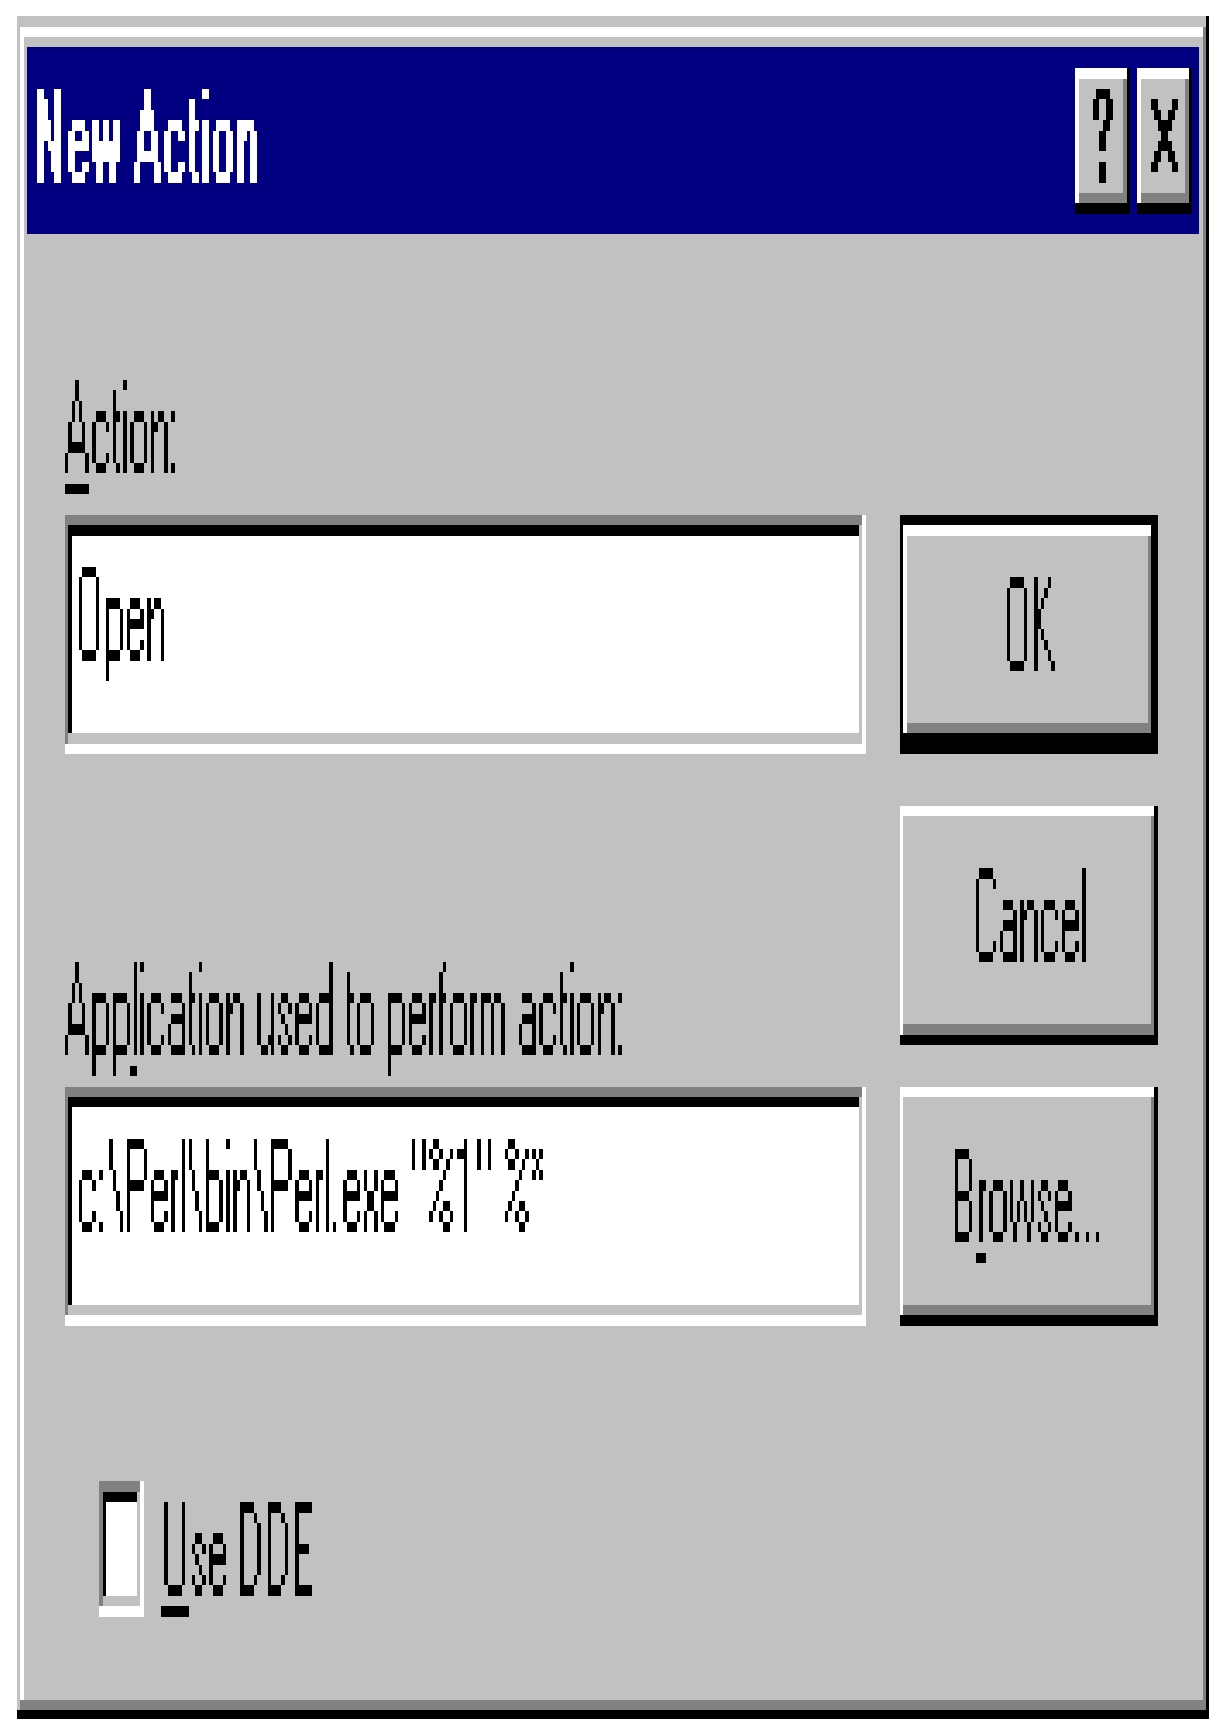
\includegraphics[bb=0mm 0mm 208mm 296mm, width=68.8mm, height=33.8mm, viewport=3mm 4mm 205mm 292mm]{image1.ps}4.   Now click New, and type Open in the Action text box, and c:\textbackslash Perl\textbackslash bin\textbackslash Perl.exe "\%1" \%* (or whatever location you chose when installing Perl) under Application used to perform action as shown below.

\noindent 

\noindent 

\noindent 

\noindent 

\noindent 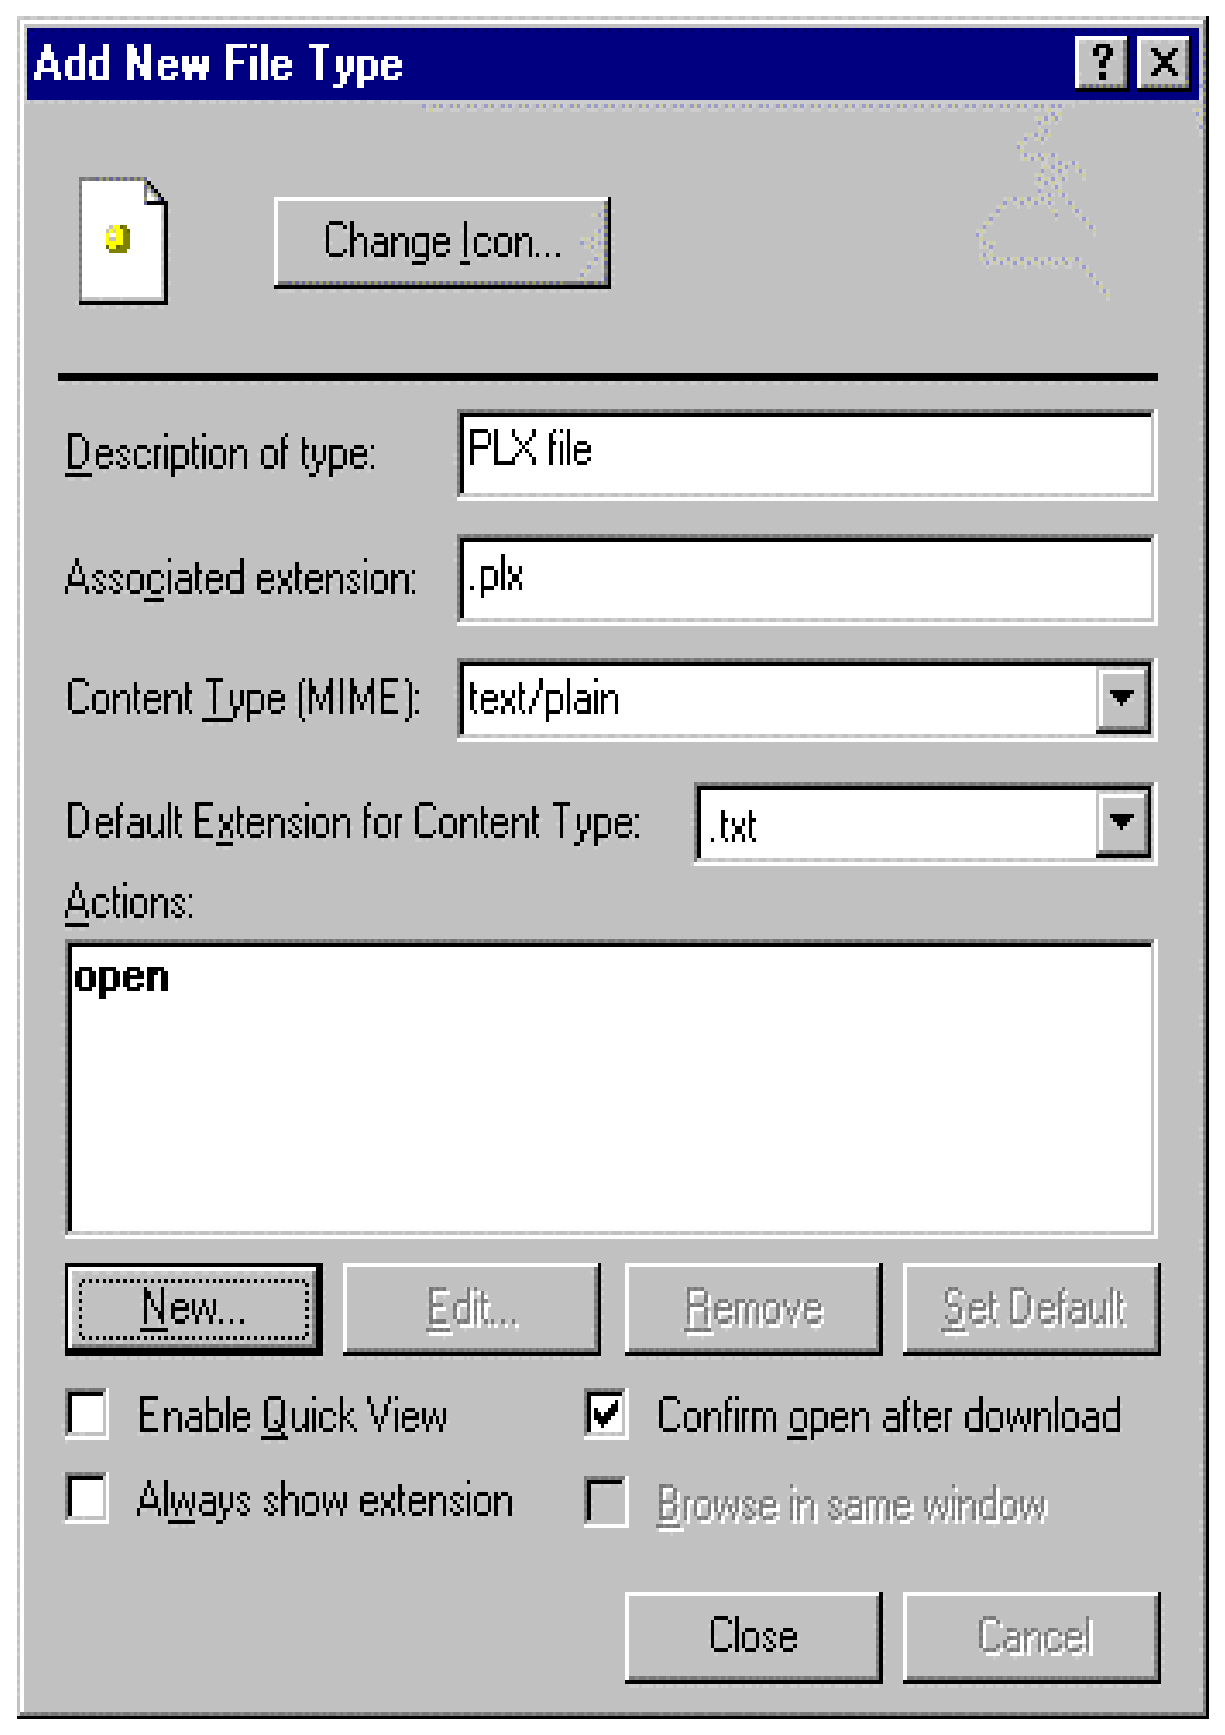
\includegraphics[bb=0mm 0mm 208mm 296mm, width=67.0mm, height=82.1mm, viewport=3mm 4mm 205mm 292mm]{image2.ps}5.   Click on OK to exit the New Action dialog, and now your screen will look something like this:

\noindent 

\noindent 

\noindent 6.   Finally,  close the Add New File Type dialog,  and  you  should  now  be  able  to  see the

\noindent 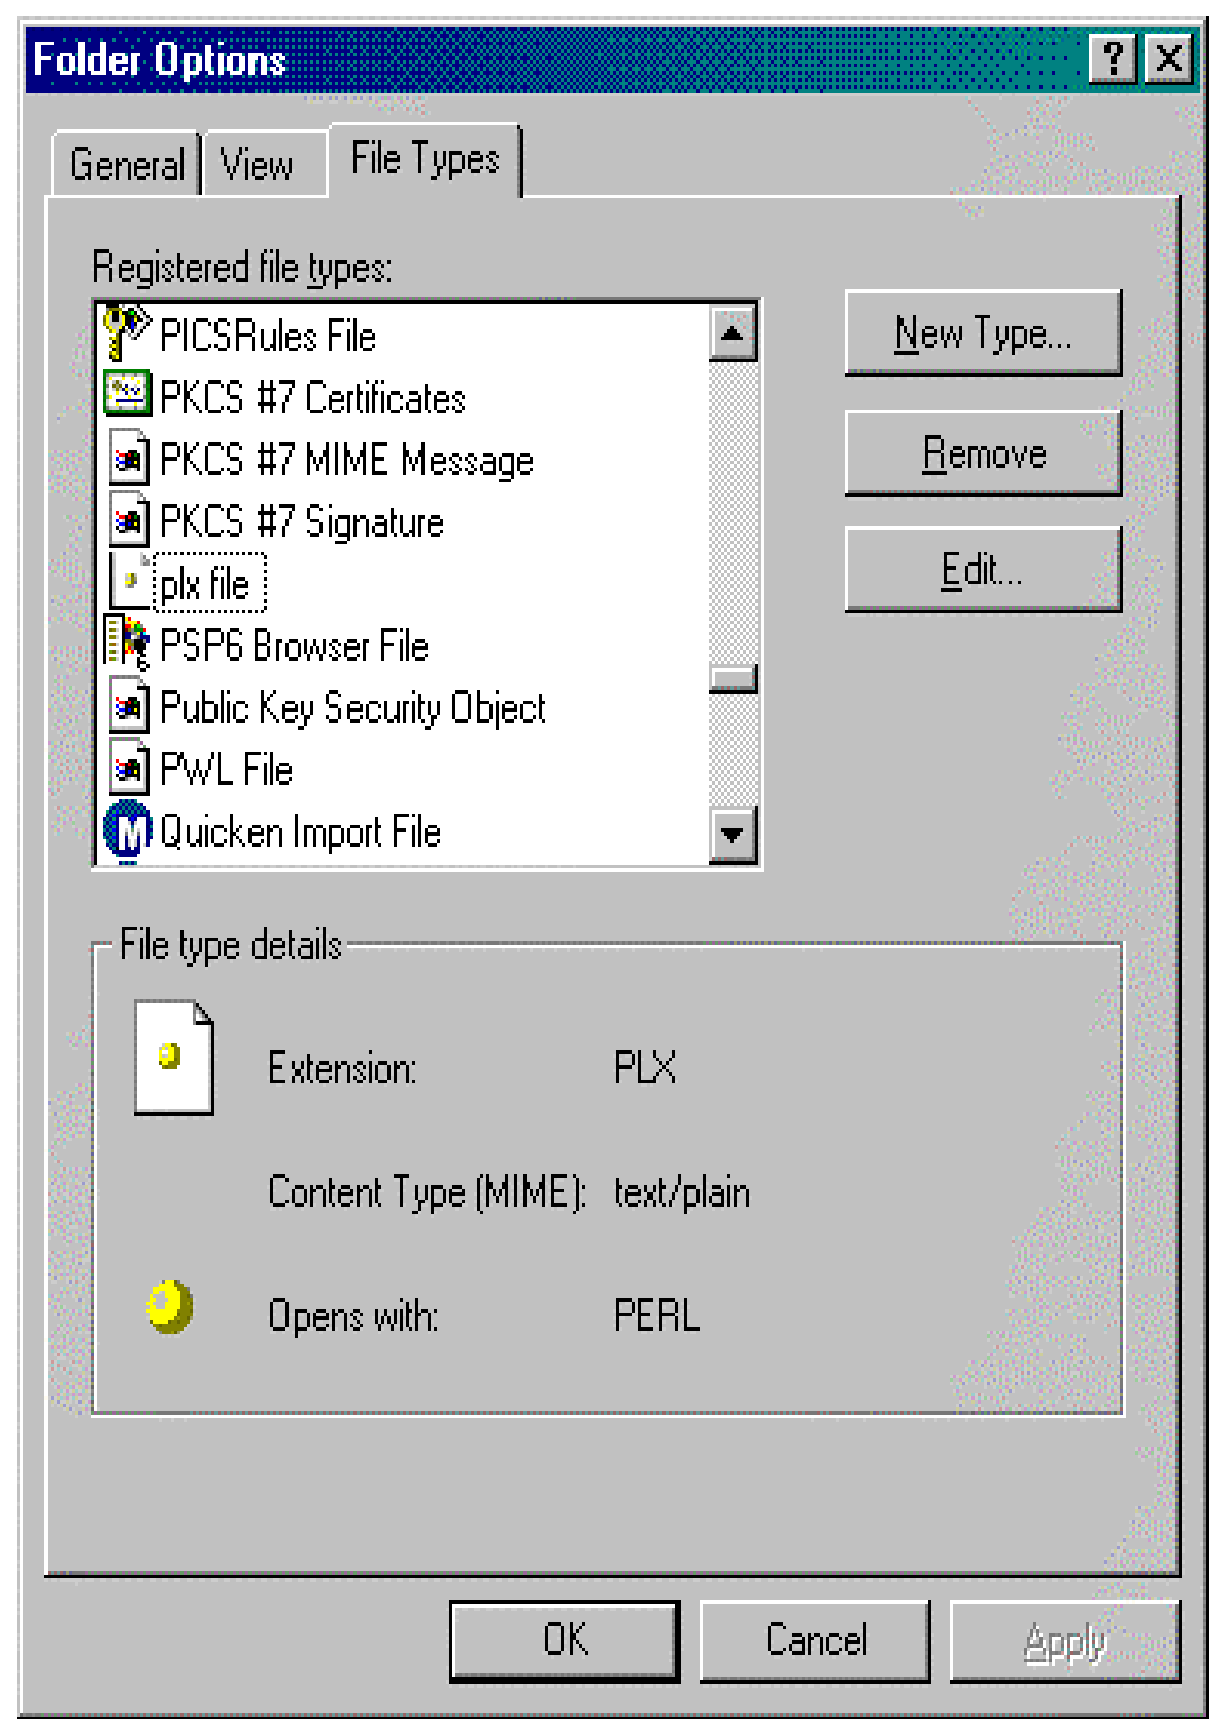
\includegraphics[bb=0mm 0mm 208mm 296mm, width=68.4mm, height=83.0mm, viewport=3mm 4mm 205mm 292mm]{image3.ps}following window:

\noindent 

\noindent 

\noindent 

\noindent 

\noindent 

\noindent 

\noindent 

\noindent 

\noindent 

\noindent 

\noindent 

\noindent 

\noindent 

\noindent 

\noindent 

\noindent 

\noindent 

\noindent 

\noindent 

\noindent 

\noindent 

\noindent 

\noindent 

\noindent 

\noindent 

\noindent 

\noindent Notice that your .plx file displays the pearl icon, which means that we are finished, and everything

\noindent will work according to plan.

\noindent 

\noindent \textit{For Windows NT / 2000 Users...}

\noindent 1.   Open the Start menu and choose \underbar{C}ontrol Panel from the \underbar{S}ettings menu. Double click on the

\noindent Folder Options control panel.

\noindent 

\noindent 2.   Select the File Types tab and hit \underbar{N}ew.

\noindent 

\noindent 3.   In the Create New Extension dialog, type PLX as your new extension.

\noindent 

\noindent 4.   Finally, select Ad\underbar{v}anced $>$$>$ and Perl File from the drop-down list that eventually appears.

\noindent 

\noindent 5.   Hit  OK,  and for  confirmation,  the  extension,  along  with  a  pearl  icon  and the  associated File Type,  'Perl File'  should have  appeared  in  the  main  list  box.  Hit  Close to  leave  the control panel.

\noindent 

\noindent How To Get Help

\noindent 

\noindent Perl comes with an excellent set of documentation. The interface to this system is through a command, itself a Perl program, called perldoc. UNIX users can also use the man command to get at the same information, but perldoc allows you to do interesting things, as you're about to see.

\noindent 

\noindent 

\noindent \textit{Perldoc}

\noindent Typing perldoc perl from a command prompt will get you the table of contents and some basic information about Perl. The pages you're probably going to use the most are the Perl FAQ and

\noindent 'perlfunc', which describes the built-in functions.

\noindent 

\noindent Because of this, perldoc has a special interface to these two pages. perldoc -f allows you to see information about a particular function, like this:

\noindent 

\noindent $>$ \textbf{perldoc -f print}

\noindent print FILEHANDLE LIST

\noindent print LIST

\noindent print   Prints a string or a comma-separated list of strings.  Returns TRUE if successful. . . .

\noindent 

\noindent Similarly, perldoc -q allows you to search the Perl Frequently Asked Questions (FAQ) for any regular expression or keyword.

\noindent 

\noindent $>$ \textbf{perldoc -q reverse}

\noindent Found in /usr/lib/perl5/5.6.0/pod/perlfaq4.pod

\noindent How do I reverse a string?

\noindent Use reverse() in scalar context, as documented in the reverse entry in the perlfunc manpage

\noindent 

\noindent \$reversed = reverse \$string;

\noindent 

\noindent Now  see  if  you  can find that question  about  commercial  Perl  support  that  I  mentioned earlier.

\noindent 

\noindent As well as the documentation pages for the language itself, whose names all start 'perl', there's an awful

\noindent lot of other documentation out there, too. The reason for this is modules: files containing Perl code that can be used to help with a certain task. Later on we'll examine what modules are available and what

\noindent they can help us do, but you should know that each Perl module, whether a core module that comes with the Perl package or one you download from the Internet, should contain its own documentation.

\noindent We'll see how that's constructed later -- for now though, know that you can use perldoc to get at this too. Here's the beginning of the documentation for the Text::Wrap module, which is used to wrap lines into paragraphs.

\noindent 

\noindent $>$ \textbf{perldoc Text::Wrap}

\noindent 

\noindent 5.6.0::Text  User Contributed Perl Documentation  Text::Wrap

\noindent 

\noindent 

\noindent NAME

\noindent Text::Wrap - line wrapping to form simple paragraphs

\noindent 

\noindent ...

\noindent 

\noindent The pages are written in a special mark-up language called 'POD' (which sounds mysterious, but in fact stands for 'Plain Old Documentation'). The perldoc utility attempts to translate this into ordinary text when you view it, but if for some reason it cannot, you may need to specify the --t option to perldoc.

\noindent If your documentation ends up looking like this:

\noindent 

\noindent 

\noindent $>$ \textbf{perldoc -q reverse}

\noindent =head1 Found in /usr/lib/perl5/5.6.0/pod/perlfaq4.pod

\noindent =head2 How do I reverse a string?

\noindent Use reverse() in scalar context, as documented in

\noindent $<$perlfunc/reverse$>$

\noindent \$reversed = reverse \$string;

\noindent 

\noindent then you will need to run perldoc --t --q reverse instead.

\noindent 

\noindent \textit{Manpages}

\noindent As well as the perldoc system, perl may well have installed its documentation in some other places as well. UNIX people can get at the standard documentation as man pages (providing the MANPATH environment variable includes the correct location), and ActiveState users should be able to find the documentation under ActivePerl \textbar  Online Documentation on the Start menu.

\noindent 

\noindent There's an exorbitant wealth of knowledge in these pages, and some are well beyond the scope of this book. Here then is a list of those relevant to this book, in roughly the order we touch on the topics in

\noindent the book, plus one or two others that are handy and may satisfy your curiosity.

\noindent 

\noindent 

\noindent \textbf{Documentation Page Subject}

\noindent 

\noindent perl Introduction to Perl, and 'cover sheet'

\noindent 

\noindent perltoc Table of contents -- what's in the other pages

\noindent 

\noindent perlfaq Index to the Frequently Asked Questions

\noindent 

\noindent perlfaq1, perlfaq2\dots 

\noindent perlfaq9

\noindent 

\noindent The Perl Frequently Asked Questions

\noindent 

\noindent perlpod Plain Old Documentation and how to write it

\noindent 

\noindent perlbook Information on Perl books

\noindent 

\noindent perlstyle Perl style guide

\noindent 

\noindent perllexwarn A guide to the new use warnings feature of Perl.

\noindent 

\noindent perlsyn Perl's syntax rules perldata Perl's data types perlvar Perl's special variables perlop Perl's built-in operators

\noindent perlunicode Perl's support for Unicode perlre Regular expression reference perlopentut Tutorial on opening files perlreftut Tutorial on using references perllol Lists of lists using references

\noindent perlref Perl references

\noindent 

\noindent 

\noindent \textbf{Documentation Page Subject}

\noindent 

\noindent perlfunc Perl's built-in functions

\noindent 

\noindent perlsub Creating subroutines

\noindent 

\noindent perlrun Run-time options to perl perlmod Perl modules -- what they are perlmodinstall How to install Perl modules perlmodlib Guide to the standard modules

\noindent perlboot Randal Schwartz's Object Oriented Tutorial

\noindent 

\noindent perltoot Tom Christiansen's Object Oriented Tutorial

\noindent 

\noindent perltootc Tom Christiansen's Object Oriented Tutorial on Classes

\noindent 

\noindent perlobj Object oriented programming in Perl

\noindent 

\noindent perlbot The Bag of Object Tricks

\noindent 

\noindent perltie A walk through tied objects

\noindent 

\noindent perlipc Talking to other programs or networks perldbmfilter Controlling how Perl writes to databases perldiag What the error messages mean perldebug Debugging Perl programs

\noindent perltrap Traps for the unwary programmer

\noindent 

\noindent perlhist Perl's development history

\noindent 

\noindent If the Perl FAQ and the various documentation pages don't help answer your question, it's time to look

\noindent for other sources of information.

\noindent 

\noindent Perl Resources

\noindent 

\noindent There is a tremendous amount of Perl information available in books and on the Internet. Let's have a look at some of the more prominent ones.

\noindent 

\noindent \textit{Websites}

\noindent On the web, the first port of call is http://www.perl.com/, the main Perl community site, run by the publisher O'Reilly. This contains some good articles of interest to the Perl community and news from Perl's major developers, as well as a wealth of links, tips, reviews, and documentation.

\noindent 

\noindent It is also home to CPAN, the Comprehensive Perl Archive Network, a collection of ready-made programs, documents, notably the latest edition of the FAQ, some tutorials, and the Far More Than Everything You Wanted To Know About (FMTEYWTKA) series of more technical notes. Most useful

\noindent of all, this site contains a huge (and they don't call it comprehensive for nothing!) collection of those Perl modules mentioned above. We'll fully cover the use of modules and some of the best ones in a later chapter.

\noindent 

\noindent 

\noindent \textbf{Because CPAN is a network of sites, there are mirror sites around the world -- the}

\noindent \textbf{CPAN multiplexer takes you to your nearest site. Find it at}

\noindent http://www.perl.com/CPAN\textbf{ (note: no trailing slash!)}

\noindent 

\noindent 

\noindent Other important Perl sites are:

\noindent 

\noindent ? http://www.perlclinic.com/ -- Paul Ingram's Perl Clinic, providing commercial Perl support and training

\noindent ? http://www.perlfaq.com/ -- an alternative, and very comprehensive, FAQ site

\noindent ? http://www.tpj.com/ -- the home of the Perl Journal

\noindent ? http://www.activestate.com/ -- the home of Perl on Windows

\noindent ? http://www.perl.org/ -- Perl Mongers, a worldwide umbrella organisation for Perl user groups

\noindent ? http://www.perlarchive.com/ - another great source of articles, tutorials and information

\noindent 

\noindent \textit{Newsgroups}

\noindent Perl is so cool it has its own Usenet hierarchy, comp.lang.perl.*. The groups in it are:

\noindent 

\noindent ? comp.lang.perl.announce for Perl-related announcements: new modules, new versions of

\noindent Perl, conferences and so on.

\noindent ? comp.lang.perl.misc for general Perl chat and questions.

\noindent ? comp.lang.perl.moderated, which requires prior registration before posting, but is excellent for sensible questions and in-depth discussion of Perl's niggly bits.

\noindent ? comp.lang.perl.modules, for discussion and queries relating to creating and using Perl modules.

\noindent ? comp.lang.perl.tk, for discussion and queries relating to the Tk graphical extensions.

\noindent 

\noindent \textit{IRC}

\noindent If you've got a more urgent mindbender, or just want to hang around like-minded individuals, come join

\noindent \#perl on Efnet (See http://www.efnet.org/). Make sure you read the channel rules (at

\noindent http://pound.perl.org/RTFM/) and the Perl documentation \textbf{thoroughly }first, though. Asking questions

\noindent about CGI or topics covered in the FAQ or the perldoc documentation is highly inflammatory behavior.

\noindent 

\noindent If that hasn't put you off, come over and say hi to me. (I have no imagination, so my nick is usually

\noindent Simon.)

\noindent 

\noindent \textit{Books}

\noindent Of course, reading stuff from the net is a great way to learn, but I can't curl up in bed with a good web site. Not until I get myself a laptop, anyway.

\noindent 

\noindent In the meantime, there are a few good treeware resources available, too. O'Reilly has published some of the definitive books on Perl -- \textit{Learning Perl }(the Llama book), \textit{Programming Perl }(the Camel book), and

\noindent the \textit{Perl Cookbook }are well known and well respected in the Perl community. Check out the book reviews pages housed at the http://www.perl.com/ and http://www.perl.org/ sites.

\noindent 

\noindent 

\noindent As for the best book for teaching yourself Perl, just keep reading...

\noindent 

\noindent 

\noindent Conventions

\noindent 

\noindent We have used a number of different styles of text and layout in the book to help differentiate between the different kinds of information. Here are examples of the styles we use and an explanation of what they mean:

\noindent 

\noindent Try It Out -- A 'Try It Out' Example

\noindent 

\noindent 'Try It Out' is our way of presenting a practical example.

\noindent 

\noindent \textit{How It Works}

\noindent Then the 'How It Works' section explains what's going on.

\noindent 

\noindent \textit{Advice, hints and background information come in an indented, italicized font like this.}

\noindent 

\noindent 

\noindent 

\noindent 

\noindent \textbf{Important bits of information that you really shouldn't ignore come in boxes like this!}

\noindent 

\noindent 

\noindent 

\noindent ? \textbf{Important Words }are in a bold typeface.

\noindent 

\noindent ? Words that appear on the screen in menus like the File or Window menu are in a similar font

\noindent to what you see on screen.

\noindent 

\noindent ? Keys that you press on the keyboard, like \textit{Ctrl }and \textit{Enter}, are in italics.

\noindent 

\noindent 

\noindent Perl code has two fonts. If it's a word that we're talking about in the text, for example, when discussing the sub greeting \{\dots \} subroutine, it's in a distinctive font. If it's a block of code that you can type in

\noindent as a program and run, then it's shown in a gray box like this:

\noindent 

\noindent sub greeting \{

\noindent print "Hello, world!\textbackslash n";

\noindent \}

\noindent 

\noindent Sometimes you'll see code in a mixture of styles, like this:

\noindent 

\noindent sub greeting \{

\noindent print "Hello, world!\textbackslash n";

\noindent \}

\noindent 

\noindent \&greeting();

\noindent 

\noindent This is meant to draw your attention to code that's new or relevant to the surrounding discussion (in the gray box), while showing it in the context of the code you've seen before (on the white background).

\noindent 

\noindent 

\noindent Where we show text to be entered at the command prompt, this will be shown as follows:

\noindent 

\noindent $>$ \textbf{perl helloworld.plx}

\noindent 

\noindent And the output from the program will be shown in the same font, but lighter:

\noindent 

\noindent Hello World!

\noindent 

\noindent Downloading the Source Code

\noindent 

\noindent As you work through the examples in this book, you might decide that you prefer to type all the code in

\noindent by hand. Many readers prefer this, because it's a good way to get familiar with the coding techniques that are being used.

\noindent 

\noindent Whether you want to type the code in or not, we have made all the source code for this book available

\noindent at our web site, at the following address:

\noindent 

\noindent http://www.wrox.com

\noindent 

\noindent If you're one of those readers who likes to type in the code, you can use our files to check the results

\noindent you should be getting. They should be your first stop if you think you might have typed in an error. If you're one of those readers who doesn't like typing, then downloading the source code from our web

\noindent site is a must! Either way, it'll help you with updates and debugging.

\noindent 

\noindent Exercises

\noindent 

\noindent At the end of each of the first eleven chapters, you'll find a number of exercises. It is highly

\noindent recommended you work through them. This book will give you the knowledge you need - but it is only through practice that you will hone your skills and get a true feel for what Perl can help you achieve.

\noindent You can find our suggested solutions to the exercises in Appendix H at the back of the book and also for download from http://www.wrox.com, but remember that there's more than one way to do it, so they're not the only ways to solve the exercises.

\noindent 

\noindent 

\noindent Errata

\noindent 

\noindent We've made every effort to make sure that there are no errors in the text or the code. However, to err is human, and as such we recognize the need to keep you informed of any mistakes as they're spotted and corrected. Errata sheets are available for all our books at http://www.wrox.com/. If you find an error that hasn't already been reported, please let us know, by emailing support@wrox.com.

\noindent 

\noindent Our web site acts as a focus for  other  information  and  support,  including  the code  from  all  our  books, sample  chapters,  previews of  upcoming  titles,  news  of  Wrox  conferences,  and articles  and  opinion  on related topics.  For a more in-depth  look  at  our  online  support  and  errata,  turn  to  Appendix J.

\noindent 

\noindent 

\noindent Customer Support

\noindent 

\noindent Our commitment to our readers doesn't stop when you walk out of the bookstore. We want you to get the most out of this book, and we provide a selection of support services for all our readers. See Appendix J for information about our support process and our community P2P mailing lists.

\noindent 

\noindent We've tried to make this book as accurate and enjoyable as possible, but what really matters is what the book actually does for you. Please let us know your views, either by returning the reply card in the back

\noindent of the book, or by emailing us at feedback@wrox.com.

\noindent  

\noindent  

\noindent  

\noindent  

\noindent 

\noindent 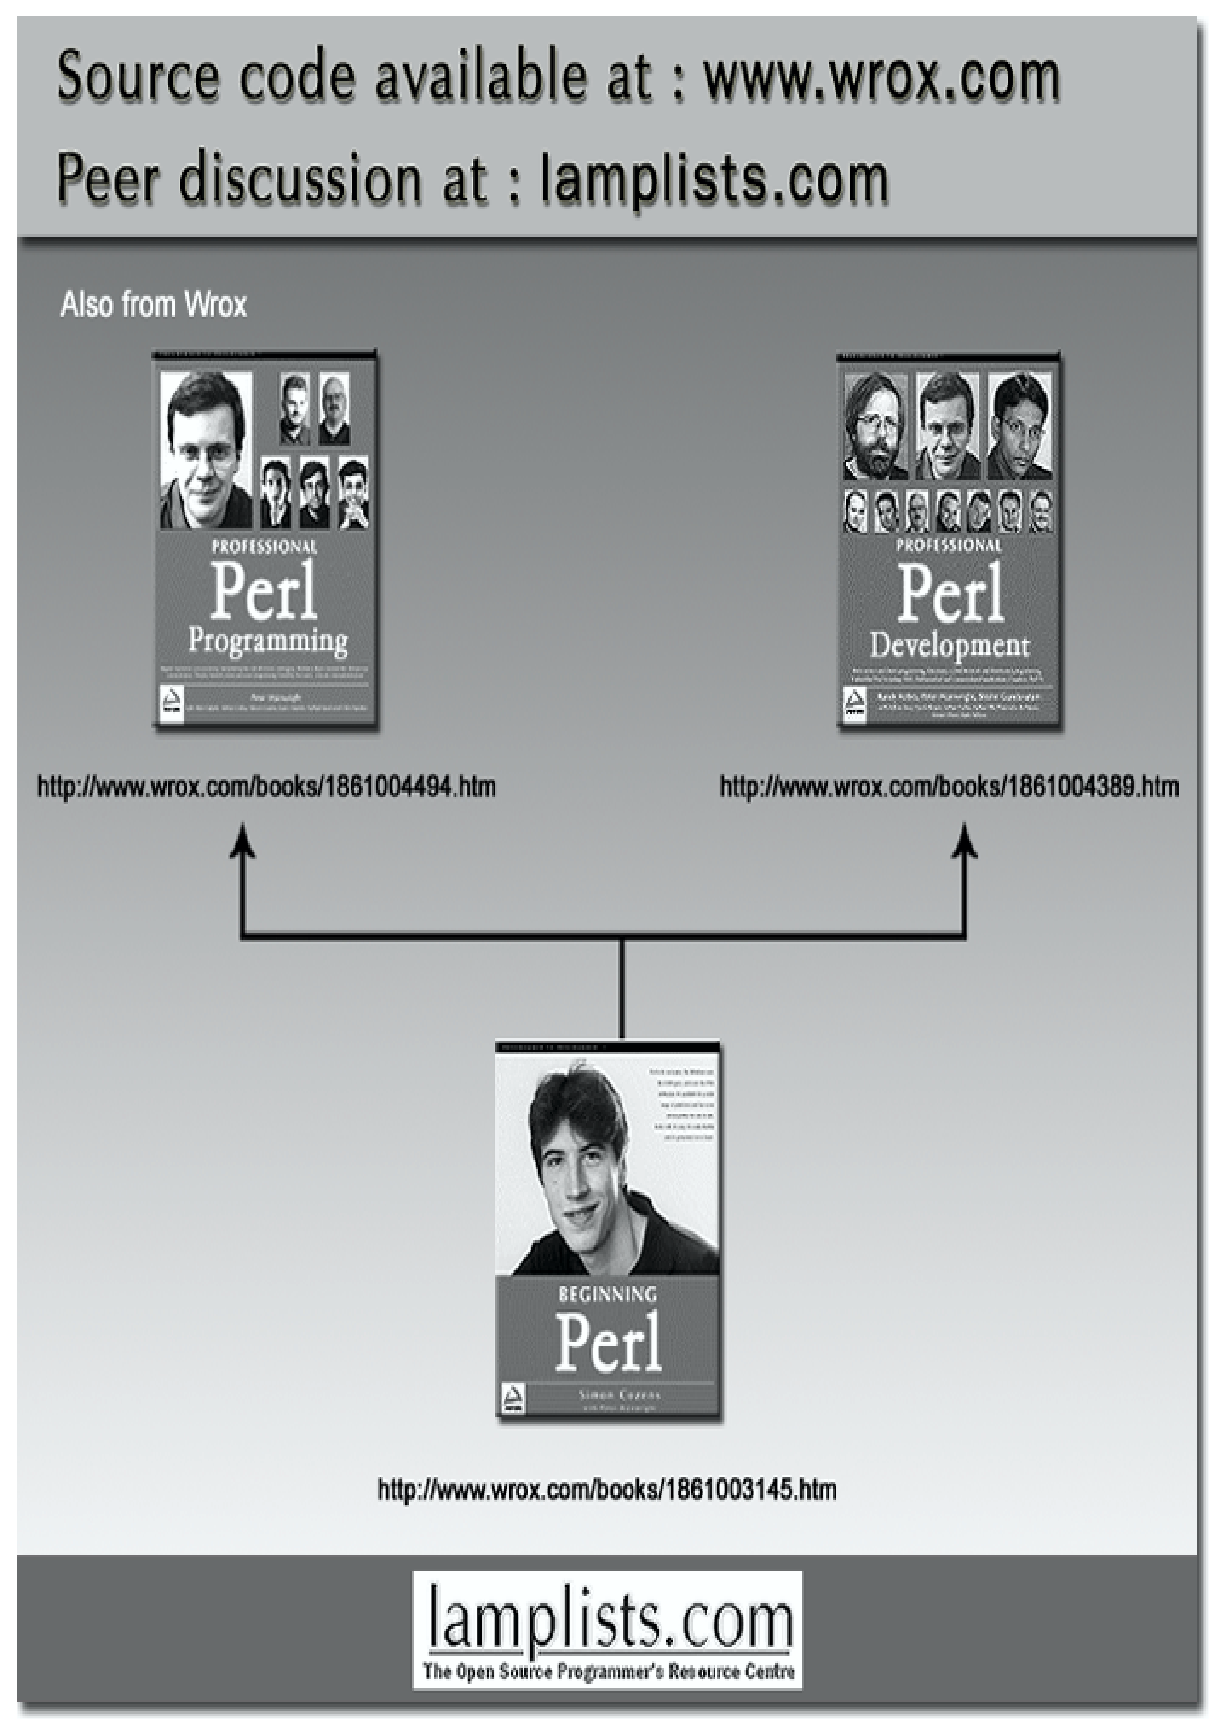
\includegraphics[bb=0mm 0mm 208mm 296mm, width=185.2mm, height=196.3mm, viewport=3mm 4mm 205mm 292mm]{image4.ps}

\noindent 

\noindent This work is licensed under the Creative Commons Attribution-NoDerivs-NonCommercial License. To view a copy of this

\noindent license, visit http://creativecommons.org/licenses/by-nd-nc/1.0 or send a letter to Creative Commons, 559 Nathan Abbott Way, Stanford, California 94305, USA.

\noindent 

\noindent The key terms of this license are:

\noindent 

\noindent Attribution: The licensor permits others to copy, distribute, display, and perform the work. In return, licensees must give the original author credit.

\noindent 

\noindent No  Derivative  Works: The licensor permits others to copy, distribute, display and perform only unaltered copies of the work -- not derivative works based on it.

\noindent 

\noindent Noncommercial: The licensor permits others to copy, distribute, display, and perform the work. In return, licensees may not use the work for commercial purposes -- unless they get the licensor's permission.


\end{document}

% == UNREGISTERED! == GrindEQ Word-to-LaTeX 2008 ==

